% -*- latex -*-
%%%%%%%%%%%%%%%%%%%%%%%%%%%%%%%%%%%%%%%%%%%%%%%%%%%%%%%%%%%%%%%%
%%%%
%%%% This TeX file is part of the course
%%%% Introduction to Scientific Programming in C++/Fortran2003
%%%% Victor Eijkhout eijkhout@tacc.utexas.edu
%%%% copyright 2017-2023
%%%%
%%%% object.tex : we get down to OOP!
%%%%
%%%%%%%%%%%%%%%%%%%%%%%%%%%%%%%%%%%%%%%%%%%%%%%%%%%%%%%%%%%%%%%%

\Level 0 {What is an object?}
\label{sec:object}

You have now learned about elementary data,
control structures,
and functions.
Ultimately, that's all there is to programming:
data and operations on them.
However, to keep your programs manageable
it is a good idea to structure them,
and recognize that you really want to talk at a higher level of abstraction.

C++ offers an important mechanism of unifying data and operations
to give a new level of abstraction:
\indextermdef{object}s belonging to \indextermdef{class}es.

\begin{mdframed}
  \begin{quotation}
    \noindent
    An object is an entity that you can request to do certain things.

    \noindent
    When designing a class, first ask yourself: `what functionality
    should the objects support'.
  \end{quotation}
\end{mdframed}

\begin{itemize}
\item
  The actions an object is capable of are the
  \emph{methods}\index{methods|see{member, function}}
  or \indextermsub{function}{member}s of the object; and
\item to make these actions possible the object probably stores
  data, the
  \indextermsub{data}{member}s.
\item
  Objects comes in \indexterm{class}es. A~class is like a datatype:
  you can make objects of a class like you make variables of a datatype.
\item
  Objects of the same class have the same methods.
  They also have the same members, but with individual values.
\end{itemize}

\begin{slide}{Definition of object/class}
  \label{sl:object-def}
  An object is an entity that you can request to do certain
  things. These actions are the
  \emph{methods},
  and to make these possible the object probably stores
  data, the
  \emph{members}.

  When designing a class, first ask yourself:\slidebreak
  `what functionality should the objects support'.

  A \indexterm{class} is a user-defined type;
  an object is an instance of that type.
\end{slide}

Classes are like datatypes in that you can declare
variables of that type,
which can then be used in expressions.
Unlike basic datatypes, they are not predefined,
so you first need to define the class before
you can make objects of that class.

\begin{itemize}
\item You need a class definition, typically placed before the main
  program.
\item (In larger programs you would put it in a
  \indextermsub{include}{file} or \indexterm{module}.)
\item You can then declare multiple objects belonging to that
  class.
\item Objects can then be used in expressions, passed as parameter, et cetera.
\end{itemize}

\begin{slide}{Objects and classes}
  \label{label:class-def}
  An object is a particular instance of a \indextermdef{class} of
  similar objects, so you need a \indextermbus{class}{definition},
  after which you define objects of that class.
\end{slide}

\Level 1 {First example: points in the plane}

In this section we will use a simple example
as an illustration of how to use object:
we are going to create a
\lstinline{Point} object, corresponding to a mathematical point
in~$\mathbb{R}^2$.

The presentation will be rather top-down:
we will more focus on what to do,
rather than how to do it.
No worries, all details will be covered in due time.

\begin{exercise}
  \label{ex:point-what}
  Thought exercise:
  what are some of the actions that a point object
  should be capable of?
\end{exercise}

The first things we are going to do with a point are to
query some of its mathematical properties.
For instance,
given a point, you could want to know its distance to the origin
or its angle with the $x$-axis.

\begin{block}{Object functionality}
  \label{sl:object-functionality}
  Small illustration: point objects.
  %
  \snippetwithoutput{functionality}{object}{functionality}
  %
  Note the `dot' notation. 
\end{block}

\begin{exercise}
  \label{ex:pointdesign}
  Thought exercise:\\
  What data does the object need to store to be able to calculate
  angle and distance to the origin?\\
  Is there more than one possibility?
\end{exercise}

Food for thought: you may be tempted  to  write methods for getting the $x$ and $y$
coordinate. However, ask yourself if those should be publicly visible methods.
Is getting the $x$ coordinate a linear algebra operation? When you have methods
such as `get the distance to the origin' or `shift this point rightward',
do you explicitly need the coordinates?

The above example used a \lstinline{Point} object without saying
how it was created.
That's what we are going to look at next.

\begin{block}{The object workflow}
  \label{sl:object-flow}
  \begin{itemize}
  \item First define the class, with data and function members:
\begin{lstlisting}
class MyObject {
  // define class members
  // define class methods
};
\end{lstlisting}
(details later)
typically before the \lstinline{main}.
  \item You create specific objects with a declaration
\begin{lstlisting}
MyObject
  object1( /* .. */ ),
  object2( /* .. */ );    
\end{lstlisting}
  \item You let the objects do things:
\begin{lstlisting}
object1.do_this();
x = object2.do_that( /* ... */ );
\end{lstlisting}
  \end{itemize}
\end{block}

Let's now introduce the details of all these steps.

\Level 1 {Constructor}
\label{sec:simple-constructor}

First we'll look at creating class objects,
and we'll stick with the point example.

Since a point can be defined by its $x,y$ coordinates,
you can imagine that
\begin{itemize}
\item
  the point object stores these coordinates, and
\item when you create a point object, you do that by
  specifying the coordinates.
\end{itemize}

Here are the relevant fragments of code:
\begin{block}{Construct an object}
  \label{sl:point-construct-use}
\begin{multicols}{2}
  The declaration of an object~\lstinline{x}
  of class \lstinline+Point+;
  the coordinates of the point are initially
  set to \n{1.5,2.5}.
\begin{lstlisting}
Point x(1.5, 2.5);
\end{lstlisting}
%
\columnbreak
%
  \lstset{style=snippetcode}
\begin{lstlisting}
class Point {
private: // data members
  double x,y;
public: // function members
  Point
    ( double x_in,double y_in ) {
      x = x_in; y = y_in;
  };
  /* ... */
};
\end{lstlisting}
\end{multicols}
\begin{tldr}
  Use the \indexterm{constructor} to create an object of a class:\\
  function with same name as the class.\\
  (but no return type!)
\end{tldr}
\end{block}

Study the implementation closely.
The class is named \lstinline{Point},
and there is something that looks like a function definition,
also named \lstinline{Point}.
However, unlike a regular function, it does not have a return type,
not even \lstinline{void}.

This function is named the \indexterm{constructor} of the class,
and it is characterized by:
\begin{itemize}
\item The constructor has the same name as the class, and
\item it looks like a function definition,
  except that it has no return type.
\end{itemize}
When you create an object,
in the manner you've seen in above examples,
you actually call this constructor.

Usually you write your own constructor,
for instance to initialize data members.
In the case of the \lstinline{class Point}
the function of the constructor is to take the coordinates
of the point and to copy them to private members of the \lstinline{Point} object.

If the object you create can have sensible default values,
you can also use a \indextermsub{default}{constructor},
which has no argument.
We will get to that below; section~\ref{sec:default-constructor}.

\Level 1 {Data members}

In the examples so far, your created a point object from its coordinates
\begin{lstlisting}
  Point oneone(1.,1.);
\end{lstlisting}
and the \lstinline{Point} object stored these coordinates.
However, this connection between outward usage and internal implementation
can be very different.
Maybe you have an application that works in polar coordinates,
in which case storing $r,\theta$ is more natural,
or at least more convenient for computation.
But you may still want to create a point from its Cartesian coordinates.

\begin{block}{Food for thought: constructor vs data}
  \label{sl:class-set}
  The arguments of the constructor imply nothing about
  what data members are stored!

  Example: create a point in \lstinline{x,y} Cartesian coordinates,
  but store \lstinline{r,theta} polar coordinates:

  \lstset{style=snippetcode}
\begin{lstlisting}
#include <cmath>
class Point {
private: // members
  double r,theta;
public: // methods
  Point( double x,double y ) {
    r = sqrt(x*x+y*y);
    theta = atan2(y/x);
  }
\end{lstlisting}
Note: no change to outward API.
\end{block}

You have now seen the \indexc{private} and \indexc{public} keywords.
These indicate the visibility of class members.

\begin{plainblock}{Member visibility}
  \begin{itemize}
  \item Keyword \indexc{private} indicates that data is internal:
    not accessible from outside the object;
    can only be used inside function members.
  \item Keyword \indexc{public} indicates that the constructor
    function can be used in the program.
  \end{itemize}
\end{plainblock}

\begin{slide}{Data access in methods}
  \label{sl:member-access-proper}
  You can access data members of other objects of the same type:
  \lstset{style=snippetcode}
\begin{lstlisting}
class Point {
private:
  double x,y;
public:
 void flip() {
    Point flipped;
    flipped.x = y; flipped.y = x;
    // more
  };
};
\end{lstlisting}
  (Normally, data members should not be accessed directly from outside an object)
\end{slide}

You may have observed that the private members are all data members,
while all the function members are public.
This is no coincidence: for now you can consider this a `best practice'.

\begin{block}{Private and public}
  \label{sl:public-private-basic}
  Best practice we will use:
\begin{lstlisting}
class MyClass {
private:
  // data members
public:
  // methods
}
\end{lstlisting}
\begin{itemize}
\item Data is private: not visible outside of the objects.
\item Methods are public: can be used in the code that uses objects.
\item You can have multiple private/public sections, in any order.
\end{itemize}
\end{block}

\Level 1 {Methods}

Methods are things you can ask your class objects to do. For instance,
in the \lstinline{Point} class, you could ask
a point to report its distance to the origin,
or you could ask it to scale its distance by some number.

Let's start with the simpler of these two: measuring the distance to the origin.
Without classes and objects, you would write a function with $x,y$ coordinates
as input,
and a single number as output
\begin{lstlisting}
float x = ..., y = ...;
float d = distance_to_origin(x,y);
\end{lstlisting}

For an object method this looks like:
\begin{lstlisting}
float x=..., y=...;
Point p( x,y );
float d = p.distance_to_origin();
\end{lstlisting}
To point out differences and similarities:
\begin{itemize}
\item
  You're still using a function with a scalar output, but
\item instead of input parameters we use the coordinates
  that are stored in the point object.
  These act as `global variables', at least within the object.
\item To apply this function to a point, we use the `dot' notation.
  You could pronounce this as `p's distance to the origin'.
  Note that this function is only available
  as applying to a point; you can not use it in other contexts.
\end{itemize}

\begin{block}{Class methods}
  \label{sl:method-define}
  Definition and use of the \lstinline{distance} function:
  
  \snippetwithoutput{pointodist}{geom}{pointodist}
\end{block}

\begin{slide}{Class methods}
  \label{sl:method-observe}
  \begin{itemize}
  \item Methods look like ordinary functions,
  \item except that they can use the data members of the class, for
    instance~\lstinline{x,y};
  \item Methods can only be used on an object with the `dot' notation.
    They are not independently defined.
  \end{itemize}
\end{slide}

\begin{exercise}
  \label{ex:vectorclass-angle}
  Add a method \lstinline{angle} to the \lstinline{Point} class.
  How many parameters does it need?

  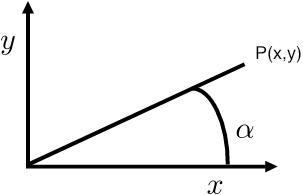
\includegraphics[scale=.2]{pointangle}

  Hint: use the function \lstinline{atan} or \lstinline{atan2}.
  \skeleton{pointclass}
\end{exercise}

\begin{exercise}
  \label{ex:manhattan}
  Make a class \lstinline{GridPoint} which can have only integer coordinates.
  Implement a function \lstinline{manhattan_distance} which gives the distance
  to the origin counting how many steps horizontal plus vertical it takes
  to reach that point.
\end{exercise}

\Level 1 {Initialization}

There are various ways of setting the initial values
of the data members of an object.

\Level 2 {Default values}

Sometimes it makes sense for objects to have default values
if nothing else is specified.
This can be done with setting default values on the data members:

\begin{block}{Member default values}
  \label{sl:class-defval}
  Class members can have default values, just like ordinary variables:
\begin{lstlisting}
class Point {
private:
  float x=3., y=.14;
public:
  // et cetera
}
\end{lstlisting}
  Each object will have its members initialized to these values.
\end{block}

\Level 2 {Initialization in the constructor}

\index{member!initializer|see{initializer, member}}

Above you saw some examples of constructors that are used
to initialize the object data.
There is more than one way to do that.

First of all, you can copy the constructor arguments
in the body of the constructor.
However, the preferred way is by using \indextermsub{member}{initializer}s,
which takes a new notation.

\begin{block}{Data initialization}
  \label{sl:contructor-init-2}
\begin{multicols}{2}
The naive way:
  \lstset{style=snippetcode}
\begin{lstlisting}
class Point {
private:
  double x,y;
public:
  Point( double in_x,
         double in_y ) {
    x = in_x; y = in_y;
  };
\end{lstlisting}
\columnbreak
The preferred way:
\verbatimsnippet{classpointinit}
\end{multicols}
\end{block}

(See section~\ref{sec:class-w-vector} for why member initializers are preferred.)

You can even save yourself from having to think of too many names:

\snippetwithoutput{classpointinitxy}{geom}{pointinitxy}

The initialization \lstinline{x(x)} should be read as
\lstinline{membername(argumentname)}.
Yes, having \lstinline{x} twice is a little confusing.

\begin{slide}{Member initializer lists}
  \label{sl:class-init}
  Other syntax for initialization:\slidenewline
  use initializer list.
  %
  \verbatimsnippet{classpointinit}
\end{slide}

\begin{slide}{Advantage of initializer list}
  \label{sl:class-init-why}
  Allows for reuse of names:
  %
  \snippetwithoutput{classpointinitxy}{geom}{pointinitxy}
\end{slide}

\Level 1 {Methods, a deeper dive}

You have just seen examples of class
\indextermdef{method}s: a function that is only defined for objects of
that class, and that has access to the private data of that object.

In exercise~\ref{ex:vectorclass-angle} you implemented an \lstinline{angle} function,
that computed the angle from the stored coordinates.
You could have made other decisions.

\begin{exercise}
  \label{ex:vectorclass-redundant}
  Discuss the pros and cons of this design:
  \lstset{style=snippetcode}
\begin{lstlisting}
class Point {
private:
  double x,y,r,theta;
public:
  Point(double xx,double yy) {
    x = xx; y = yy;
    r = // sqrt something
    theta = // something trig
  };
  double angle() { return alpha; };
};
\end{lstlisting}
\end{exercise}

By making these functions public, and the data members
private, you define an \acf{API} for the class:
\begin{itemize}
\item You are defining operations for that class; they are the only
  way to access the data of the object.
\item The methods can use the data of the object, or alter it. All
  data members, even when declared \indexc{private}, are global to the methods.
\item  Data members declared \indexc{private} are not accessible from outside the
  object.
\end{itemize}

\begin{review}
  \label{rev:class-meth-data}
  T/F?
  \begin{itemize}
  \item A class is primarily determined by the data it stores.
    \slackpollTF+Class determined by its data+
  \item A class is primarily determined by its methods.
    \slackpollTF+Class determined by its methods+
  \item If you change the design of the class data,
    you need to change the constructor call.
    \slackpollTF+Change data, change constructor proto too+
  \end{itemize}
\end{review}

\begin{slide}{Functions on objects}
  \label{sl:obj-func}
  %\let\codesize\scriptsize
  \snippetwithoutput{pointfunc}{geom}{pointfunc}
  We call such internal functions `methods'.\\
  Data members, even \lstinline{private}, are global to the methods.
\end{slide}

Now let's look at some different types of objects.
This is an informal classification, not necessarily
corresponding to defined concepts in the C++~standard.

\Level 2 {Changing state}

Objects usually have data members that maintain the
\emph{state}\index{object!state of} of the object.
By changing the
values of the members you change the state of the object.
Doing so is
usually done through a method.

\begin{block}{Methods that alter the object}
  \label{sl:obj-func-on}
  For instance, you may want to scale a vector by some amount:
  %
  \snippetwithoutput{pointscaleby}{geom}{pointscaleby}
\end{block}

\begin{exercise}
  \label{ex:shift-point-right}
  Implement a method \lstinline+shift_right+ for the \lstinline{Point} class.
\end{exercise}

\begin{exercise}
  \label{ex:polar-rotate}
  Take the \lstinline{Point} class design that uses polar coordinates
  (see above).
  Implement a \lstinline{rotate} method.

  There is a subtlety here. Hint: imagine rotating a point
  sufficiently many times.
\end{exercise}

\Level 2 {Methods that return objects}

The methods you have seen so far only returned elementary
datatypes. It is also possible to return an object, even from the same
class. For instance, instead of scaling the members of a vector object, you
could create a new object based on the scaled members:
%
\snippetwithoutput{pointscale}{geom}{pointscale}

\begin{slide}{Methods that create a new object}
  \label{sl:obj-return}
  \snippetwithoutput{pointscale}{geom}{pointscale}
  Note the `anonymous object' in the assignment
\end{slide}

\begin{block}{Anonymous objects}
  \label{sl:obj-return-move}
Create a point by scaling another point:
\begin{lstlisting}
new_point = old_point.scale(2.81);
\end{lstlisting}

  Two ways of handling the \lstinline{return} statement:
  \lstset{style=snippetcode}
  \begin{multicols}{2}
    \footnotesize
    Naive:
    \verbatimsnippet{pointscaleimpl1}
    Creates point, copies it to \lstinline+new_point+
    \par\vfill \columnbreak
    Better:
    \verbatimsnippet{pointscaleimpl2}
    Creates point, moves it directly to \lstinline+new_point+
  \end{multicols}
  `move semantics' and `copy elision':\slidebreak
  compiler is pretty good at avoiding copies
\end{block}

\Level 1 {Default constructor}
\label{sec:default-constructor}

You have now seen some examples of classes and their constructors.
These constructors took arguments that set the initial \indexterm{state} of the object.

However, if your objects have sensible default values, you can use a
\indextermsubdef{default}{constructor}.
For example:

\begin{block}{Using the default constructor}
  \label{sl:no-construct-default}
  No constructor explicitly defined;\\
  You recognize the default constructor in the main by the fact that an object
  is defined without any parameters.

  \snippetwithoutput{defaultno}{object}{defaultno}
\end{block}

You can define a default constructor yourself,
but the previous example had a
\emph{defaulted}\index{constructor!default!defaulted} default constructor:
it acted like it had a constructor
\begin{lstlisting}
IamZero() {};
\end{lstlisting}

Bear this in mind as you study the following code:
%
\verbatimsnippet{pointdef2}
%
With the \lstinline{Point} class (and its constructor) as given before:
\verbatimsnippet{pointodist}
this will give an error message during compilation. The reason is
that 
\begin{lstlisting}
Point p2;
\end{lstlisting}
calls the default constructor. Now that you have defined your own
constructor, the default constructor no longer exists. So you need to
define it explicitly:
%
\verbatimsnippet{pointdef1}
%
You now have a class with two constructors.
The compiler will figure out which one to use.
This is an example of \emph{polymorphism}\index{polymorphism!of constructors}.

You can also indicate somewhat more explicitly that the
\emph{defaulted default constructor}\index{constructor!default!defaulted} 
needs to exist:
\verbatimsnippet{defaulteddefault}

\begin{slide}{Default constructor}
  \label{sl:obj-def-construct1}

  Refer to point definition:~\ref{sl:point-construct-use}\\
  Consider this code that looks like variable declaration,
  but for objects:
\begin{lstlisting}
Point p1(1.5, 2.3);
Point p2;
p2 = p1.scaleby(3.1);
\end{lstlisting}

  Compiling gives (g++; different for intel):
\begin{lstlisting}
pointdefault.cxx: In function 'int main()':
pointdefault.cxx:32:21: error: no matching function for call to
                'Point::Point()'
\end{lstlisting}
\end{slide}

\begin{slide}{Default constructor}
  \label{sl:obj-def-construct2}
  The problem is with \lstinline{p2}:
\begin{lstlisting}
Point p1(1.5, 2.3);
Point p2;
\end{lstlisting}
\begin{itemize}
\item \lstinline{p1} is created with the constructor;
\item \lstinline{p2} uses the default constructor:
\begin{lstlisting}
Point() {};
\end{lstlisting}
\item as soon as you define a constructor, the default constructor
  goes away;
\item you need to redefine the default constructor:
  \verbatimsnippet{pointdef1}
  (but only if you really need it.)
\end{itemize}
\end{slide}

\begin{slide}{Other way}
  \label{sl:obj-def-construct2a}
  \verbatimsnippet{defaulteddefault}  
Also:
\begin{lstlisting}
  Point() = delete;
\end{lstlisting}
to disable.
\end{slide}

\begin{remark}
  The default constructor has `empty parentheses', but you use
  it specifying no parentheses.
  What would happen if you specified empty parentheses when you create an object?
  
  \verbatimsnippet{constructparen}

\begin{verbatim}
constructparen.cxx:24:12: warning: 
empty parentheses interpreted as a function declaration
  MyClass y();
           ^
constructparen.cxx:24:12: note:
 remove parentheses to declare a variable
  MyClass y();
           ^
1 warning generated.  
\end{verbatim}
\end{remark}

\Level 1 {Data member access; invariants}

You may have noticed the keywords \indexc{public} and
\indexc{private}. We made the data members private, and the
methods public.
The C++ language also has the \indextermtt{struct} construct,
inherited from~C.
In that one, data members are (by default) public. Why don't we do that here?

\begin{multicols}{2}
Struct data is public:
\begin{lstlisting}
struct Point {
  double x;
};
int main() {
  Point andhalf;
  andhalf.x = 1.5;
}
\end{lstlisting}

\columnbreak

\begin{lstlisting}
class Point {
public: // Bad! Idea!
  double x;
};
int main() {
  Point andhalf;
  andhalf.x = 2.6;
}
\end{lstlisting}
\end{multicols}

Objects are really supposed to be accessed through their functionality.
While you could write methods such as \lstinline+get_x+,
(this is called an \indextermdef{accessor};
see also section~\ref{sec:const-overload} for some subtleties)
to get the $x$ coordinate,
ask yourself if that makes sense.
If you need the $x$ coordinate to shift the point rightward,
write a \lstinline+shift_right+ method instead.

\begin{block}{Public versus private}
  \label{sl:interfaceimpl}
  \begin{itemize}
  \item Interface: \indexc{public} functions that determine the
    functionality of the object; effect on data members is secondary.
  \item Implementation: data members, keep \indexc{private}: they
    only support the functionality.
  \end{itemize}
  This separation is a Good Thing:
  \begin{itemize}
  \item Protect yourself against inadvertent changes of object data.
  \item Possible to change implementation without rewriting calling code.
  \end{itemize}
\end{block}

You should not write access functions lightly: you should first think
about what elements of your class should conceptually be inspectable
or changeable by the outside world.  Consider for example a class
where a certain relation holds between members. In that case only
changes are allowed that maintain that relation.
It is sometimes said that a class satisfies an \indexterm{invariant}.

You already saw this phenomenon in action in exercise~\ref{ex:polar-rotate}.
What was the invariant there?
Let's consider another example of the need of maintaining an invariant.

\begin{block}{Access gone wrong}
  \label{sl:privatenogoo}
  We make a class for points on the unit circle
  %
  \lstset{style=snippetcode}
  \verbatimsnippet{unitpointdef}
  %
  You don't want to be able to change just one of \lstinline{x,y}!\\
  In general: enforce invariants on the members.
\end{block}

Section~\ref{sec:cpp-accessor} has some further discussion on ways
of directly accessing internal data.

\Level 1 {Examples}

So far, we have looked at examples of objects that represent
`object-like' things in the real world.
However, we can also make objects for things
that are more abstract.
In the next example, we look at `infinite objects',
such as the set of all integers.
Clearly, there is no way to store the data of such object,
but the crucial question here is: what are the methods
for an object that is the set of all integers?
One possible design is that you could ask this object
`give me the next integer'.

\begin{block}{Classes for abstract objects}
  \label{sl:intstream}
  Objects can model fairly abstract things:
  %
  \snippetwithoutput{integerstream}{object}{stream}
\end{block}

\begin{exercise}
  \label{ex:mult-two}
  \begin{itemize}
  \item
    Write a class \lstinline{multiples_of_two} where every call of
    \lstinline{next} yields the next multiple of two. 
  \item Write a class \lstinline{multiples} used as follows:
\begin{lstlisting}
multiples multiples_of_three(3);      
\end{lstlisting}
  where the \lstinline{next} call gives the next multiple of the
  argument of the constructor.
  \end{itemize}
  \skeleton{stream}
\end{exercise}

\begin{exercise}
  If you are doing the prime project (chapter~\ref{ch:prime}),
  now is a good time to do exercise in section~\ref{sec:prime-seq-class}.
\end{exercise}

% {Relations between classes}
%\SetBaseLevel 1
\input inheritance
%\SetBaseLevel 0

\begin{exercise}
  If you are doing the geometry project,
  this is a good time to do the exercises in section~\ref{ex:pointfunc}.
\end{exercise}

\Level 0 {More about constructors}

\Level 1 {Delegating constructors}
\label{sec:construct-delegate}

If you have two constructors where one is a special case of the other,
there is an elegant mechanism for expressing that:
\indextermsubdef{delegating}{constructor}s.

As an example, consider a class that contains a vector,
and you want to set that vector in the constructor.
We could implement that as:
\begin{lstlisting}
class HasVector {
private:
  vector<int> values;
public:
  HasVector( vector<int> initvalues )
  : values( initvalues ) {};
\end{lstlisting}
Now suppose we want the possibility that
the vector of initial values
is only the front part of the stored vector.
Now we need a constructor that accepts
the initial values, and an integer indicating
the finished size.
\begin{lstlisting}
  HasVector( vector<int> init,int size )
  : values( vector<int>(size) ) {
    int loc=0;
    for ( auto i : init )
      values[loc++] = i;
  };
\end{lstlisting}
(Question: this constructor is somewhat dangerous.
What is the problem and how would you guard against it?)

We can now let the first constructor delegate to the more general one:
\begin{lstlisting}
  HasVector( vector<int> init )
  : HasVector( init,init.size() ) {};
\end{lstlisting}
Here we used the colon-notation to `delegate' the constructor:
one constructor is expressed in terms of another.
(Question: in the context of classes, what are
two other uses of the colon-notation?)

Everything together:
\begin{lstlisting}
class HasVector {
private:
  vector<int> values;
public:
  HasVector( vector<int> init )
  : HasVector( init,init.size() ) {};
  HasVector( vector<int> init,int size )
  : values( vector<int>(size) ) {
    int loc=0;
    for ( auto i : init )
      values[loc++] = i;
  };
\end{lstlisting}

\Level 1 {Copy constructor}
\label{sec:copy-constructor}

Just like the default constructor which is defined if you don't define
an explicit constructor, there is an implicitly defined
\indextermsubdef{copy}{constructor}\index{copy constructor|see{constructor, copy}}.
%
There are two ways you can do a copy, and they
invoke two slightly different constructors:
\begin{lstlisting}
my_object y(something); // regular or default constructor
my_object x(y);         // copy constructor
my_object x = y;        // copy assignment constructor
\end{lstlisting}
Usually the copy constructor that is implicitly defined does the right
thing: it copies all data members. (If you want to define your own copy
constructor, you need to know its prototype. We will not go into that.)

As an example of the copy constructor in action,
let's define a class that stores an integer as data member:
%
\verbatimsnippet{classwithcopy}
%
The following code shows that the data got copied over:
%
\snippetwithoutput{classwithcopyuse}{object}{copyscalar}

\begin{slide}{Copy constructor}
  \label{sl:class-copy}
  \begin{multicols}{2}
    \begin{itemize}
    \item  Default defined copy and `copy assignment' constructors:
\begin{lstlisting}
some_object x(data);
some_object y = x;
some_object z(x);
\end{lstlisting}
    \item They copy an object:
      \begin{itemize}
      \item simple data, including pointers
      \item included objects recursively.
      \end{itemize}
    \item You can redefine them as needed.
    \end{itemize}
    \vfill\columnbreak
  \lstset{style=snippetcode}
    \verbatimsnippet{classwithcopy}
  \end{multicols}
\end{slide}

\begin{slide}{Copy constructor in action}
  \label{sl:class-copy-out}
  \snippetwithoutput{classwithcopyuse}{object}{copyscalar}
\end{slide}

\begin{block}{Copying is recursive}
  \label{sl:class-copy-vector}
  Class with a vector:
  \lstset{style=snippetcode}
  \verbatimsnippet{classwithcopyvector}
  Copying is recursive, so the copy has its own vector:
  \snippetwithoutput{classwithcopyvectoruse}{object}{copyvector}
\end{block}

\Level 1 {Destructor}
\label{sec:destructor}

Just as there is a constructor routine to create an object, there is a
\indextermdef{destructor} to destroy the object.
As with the case of the default constructor, there is a default
destructor, which you can replace with your own.

A destructor can be useful if your object contains dynamically created
data: you want to use the destructor to dispose of that dynamic data
to prevent a \indextermbus{memory}{leak}. Another example is closing
files for which the \indextermbus{file}{handle} is stored in the object.

The destructor is typically called without you noticing it. For
instance, any statically created object is destroyed when the control
flow leaves its scope.

Example:
%
\snippetwithoutput{destructor}{object}{destructor}

\begin{slide}{Destructor}
  \label{sl:class-destruct}
  \begin{itemize}
  \item Every class \lstinline{myclass} has a \emph{destructor} \lstinline{~myclass}
    defined by default.
  \item The default destructor does nothing:
\begin{lstlisting}
~myclass() {};
\end{lstlisting}
\item A destructor is called when the object goes out of scope.\\
  Great way to prevent memory leaks: dynamic data can be released
  in the destructor. Also: closing files.
\end{itemize}
\end{slide}

\begin{slide}{Destructor example}
  \label{sl:class-destruct-ex1}
  Just for tracing, constructor and destructor do \lstinline{cout}:
  %
  \lstset{style=snippetcode}
  \verbatimsnippet{destructor}
\end{slide}

\begin{slide}{Destructor example}
  \label{sl:class-destruct-ex2}
  Destructor called implicitly:
\snippetwithoutput{destructoruse}{object}{destructor}
\end{slide}

\begin{exercise}
  \label{ex:destruct-trace}
  Write a class
\begin{lstlisting}
class HasInt {
private:
  int mydata;
public:
  HasInt(int v) { /* initialize */ };
  ...
}
\end{lstlisting}
used as
%
\answerwithoutput{destructexcall}{object}{destructexercise}
\end{exercise}

\begin{block}{Destructors and exceptions}
  \label{sl:exceptobj}
  The destructor is called when you throw an exception:
  %
  \snippetwithoutput{exceptdestruct}{object}{exceptdestruct}
\end{block}

\Level 0 {Advanced topics}

\Level 1 {Static variables and methods}
\label{sec:class-static}

Class members prefixed with \indexcdef{static} behave as if
they are not unique to each object of that class,
but shared between them.

The standard use for this is to count how many objects
of a class have been created.
The constructor would increment this static variable
and assign it to a private variable:
\begin{lstlisting}
Thing::Thing() {
  mynumber = n_things++; };
\end{lstlisting}

Declaring the static variable takes the keywords
\indexc{static} and \indexc{inline}:
\begin{lstlisting}
class Thing {
private:
  static inline int n_things=0; // global count
  int mynumber; // who am I?
\end{lstlisting}

\begin{slide}{Static variables}
  \label{sl:static-var}
Static variable exists once per class, not per object:
\begin{lstlisting}
class Thing {
private:
  static inline int n_things=0; // global count
  int mynumber; // who am I?
\end{lstlisting}
increase in constructor:
\begin{lstlisting}
Thing::Thing() {
  mynumber = n_things++; };
\end{lstlisting}
\end{slide}

\Level 2 {Static methods}

If you want to query the above static variables
you can of course query them from any particular object,
since they all have the same value.
However, you can define a static method:
\begin{lstlisting}
class Thing {
public:
  static int number_of_things() { return n_things; };
\end{lstlisting}
and this method can be called on the class itself;
\begin{lstlisting}
  cout << "Number of things: " << Thing::number_of_things() << '\n';
\end{lstlisting}

\Level 2 {Legacy syntax for initialization}

Prior to \cppstandard{17}, initializing the static variable was
done in a strange way. Currently, by adding the keyword \indexc{inline},
you can write:

\snippetwithoutput{staticclass}{object}{static}

\begin{comment}
  \Level 1 {Static members}
  \begin{block}{Static class members}
    \label{sl:static-member}
    A static member acts as if it's shared between all objects.\\
    (Note: C++17 syntax)
    \snippetwithoutput{classstatic17}{link}{static17}
  \end{block}
\end{comment}

In case you come across it in legacy code,
there is the C++11 syntax for static class members:

\begin{block}{Static class members, C++11 syntax}
  \label{sl:static-member11}
  \lstset{style=snippetcode}
  \verbatimsnippet{classstatic11}
\end{block}

\Level 1 {Class signatures}
\label{sec:class-decl-defn}

For purposes of organizing your code,
you may sometimes not want to include the full code of a method,
for instance in a header file.
This is the distinction between a \indexterm{declaration}
and \indexterm{definition}.

You have seen this with functions:
\begin{lstlisting}
  float f(int);
\end{lstlisting}
is the \indexterm{declaration} of a function,
stating the name of the function, the types of the input parameters
and the type of the return result.
(This is sometimes also called the `signature' or `prototype' or `header'
of the function.)
On the other hand
\begin{lstlisting}
  float f(int n) { return sqrt(n); }
\end{lstlisting}
is the \indexterm{definition} of the function, giving its full code.

Similarly, you can write class declaration, giving only the
data members and signatures of the class methods,
and specify the full method later or elsewhere.
This can for instance happen if you split your program over multiple files;
see chapter~\ref{ch:proto} and in particular section~\ref{sec:class-header-file}.

\begin{multicols}{2}
  Declaration:
\begin{lstlisting}
class Point {
private:
  float x,y;
public:
  Point(float x,float y);
  float distance();
};
\end{lstlisting}
\columnbreak
Definition:
\begin{lstlisting}
Point::Point()
  : x(x),y(y) {};
float Point::distance() {
  return sqrt( x*x + y*y );
};
\end{lstlisting}
\end{multicols}
\begin{itemize}
\item Methods, including constructors, are only given by their function header
  in the class definition.
\item Methods and constructors are then given their full definition elsewhere
  with
  `classname-double-colon-methodname' as their name.
\item (qualifiers like \lstinline{const} are given in both places.)
\end{itemize}

\Level 1 {Returning by reference}

\prerequisite{sec:class-ref}

With all the above discussion of the \ac{API} abstracting away from internals,
sometimes you really want to access the internals of an object directly.
The simplest solution is to return a copy:
\begin{lstlisting}
class Foo {
private:
  int x;
public:
  int the_x() { return x; };
};
\end{lstlisting}
There are two problems with this:
\begin{itemize}
\item
  Returning a copy can be expensive if the internal data is a big object; and
\item 
  Maybe you actually want to alter the internal data.
\end{itemize}

So we have two scenarios:
\begin{itemize}
\item you want to get a reference to a data member, in order to alter it;
\item you want to get a reference to a data member because copying is expensive,
  but you will not alter it.
\end{itemize}

First we show the general mechanism of returning
a reference to private data.

\begin{block}{Direct alteration of internals}
  \label{sl:obj-return-ref}
  Return a reference to a private member:
  \lstset{style=snippetcode}
\begin{lstlisting}
class Point {
private:
  double x,y;
public:
  double &x_component() { return x; };
};
int main() {
  Point v;
  v.x_component() = 3.1;
}
\end{lstlisting}
Only define this if you need to be able to alter the internal entity.
\end{block}

Next we show a mechanism that can be considered a performance optimization
to this: we return a reference to private data, but in such a way
that the calling side can not alter it.

\begin{block}{Reference to internals}
  \label{sl:obj-return-const-ref}
  Returning a reference saves you on copying.\\
  Prevent unwanted changes by using a `const reference'.
  \lstset{style=snippetcode}
\begin{lstlisting}
class Grid {
private:
  vector<Point> thepoints;
public:
  const vector<Point> &points() const {
    return thepoints; };
};
int main() {
  Grid grid;
  cout << grid.points()[0];
  // grid.points()[0] = whatever ILLEGAL
}
\end{lstlisting}
\end{block}

\Level 1 {Accessor functions}
\label{sec:cpp-accessor}

It is a good idea to make the data in an object private,
so that you can control who has outside access to it.
\begin{itemize}
\item Sometimes this private data is auxiliary, and there is no reason
  for outside access.
\item Sometimes you do want outside access, but you want to precisely
  control how.
\end{itemize}

Accessor functions:
\begin{lstlisting}
class thing {
private:
 float x;
public:
 float get_x() { return x; };
 void set_x(float v) { x = v; }
};
\end{lstlisting}
This has advantages:
\begin{itemize}
\item You can print out any time you get/set the value; great for
  debugging:
\begin{lstlisting}
void set_x(float v) {
  cout << "setting: " << v << endl;
  x = v; }
\end{lstlisting}
\item You can catch specific values: if \lstinline{x} is always supposed to be
  positive, print an error (throw an exception) if non-positive.
\end{itemize}

Having two accessors can be a little clumsy. Is it possible to use the
same accessor for getting and setting?

\begin{block}{Setting members through accessor}
  \label{sl:setmember}
  %
  Use a single accessor for getting and setting:

  \snippetwithoutput{objaccessref}{object}{accessref}
  %
  The function \lstinline{xvalue} returns a reference to the internal
  variable~\lstinline{x}.
\end{block}

Of course you should only do this if you want the internal variable to
be directly changeable!

\Level 1 {Polymorphism}

You can have multiple methods with the same name, as long as they can
be distinguished by their argument types. This is known as \indexterm{polymorphism};
see section~\ref{sec:polyfunc}.

\Level 1 {Operator overloading}
\label{sec:operatordef}

Instead of writing 
\begin{lstlisting}
myobject.plus(anotherobject)
\end{lstlisting}
you can actually redefine the \lstinline{+} operator so that
\begin{lstlisting}
myobject + anotherobject
\end{lstlisting}
is legal. This is known as \indextermbusdef{operator}{overloading}:
you give your own definition of common arithmetic operators.

\begin{block}{Operator overloading}
  \label{sl:object-operator}
  Syntax:
\begin{lstlisting}
<returntype> operator<op>( <argument> ) { <definition> }
\end{lstlisting}
For instance:
%
\snippetwithoutput{pointmultop}{geom}{pointmult}
%
Can also:
\begin{lstlisting}
void Point::operator*=(double factor);
\end{lstlisting}
\end{block}

\begin{exercise}
  Write a \lstinline{Fraction} class, and define the arithmetic operators on it.

  Define both the \n{+} and \n{+=} operators. Can you use one of them
  in defining the other?
\end{exercise}
\begin{exercise}
  If you know about templates, you can do the exercises in section~\ref{sec:poly-template}.
\end{exercise}

\Level 2 {Functors}

A special case of operator overloading is
\index{operator!overloading!of parentheses}%
\emph{overloading the parentheses}. This makes an object look like a
function; we call this a \indextermdef{functor}.

Simple example:
%
\snippetwithoutput{printfunctor}{object}{functor}

\begin{exercise}
  \label{ex:functor2}
  Extend that class as follows: instead of printing the argument
  directly, it should print it multiplied by a scalar. That scalar
  should be set in the constructor. Make the following code work:
  %
  \answerwithoutput{functortworun}{object}{functor2}
  %
  (The \lstinline{for_each} is part of \indextermtt{algorithm})
\end{exercise}


\Level 2 {Object outputting}
\label{sec:cout-object}

Wouldn't it be nice if you could
\begin{lstlisting}
MyObject x;
cout << x << '\n';
\end{lstlisting}
The reason this doesn't work, is that the `double less'
is a binary operator, which is not defined
with your class as second operand.

See section~\ref{sec:lessless} for the solution.

\Level 2 {Comparisons and the `spaceship' operator}

In section~\ref{sec:operatordef} above we discussed operator overloading.
In particular, you can overload the comparison operators \n{<,=,>} et cetera.
This quickly becomes a lot of work: there are six different operators.

The \cppstandard{20} standards has simplified this with
the \indexterm{spaceship operator}.

\verbatimsnippet{spaceshipless}

\Level 1 {Constructors and contained classes}

Suppose we have a class where each object contains
another object of some non-trivial class.
Now we have to be aware of how the creation of the
outer object relates to that of the inner.

\begin{block}{Constructors and contained classes}
  \label{sl:construct-contained1}
  Finally, if a class contains objects of another class,
  \lstset{style=snippetcode}
\begin{lstlisting}
class Inner {
public:
  Inner(int i) { /* ... */ }
};
class Outer {
private:
  Inner contained;
public:
};
\end{lstlisting}
\end{block}

then

\begin{block}{When are contained objects created?}
  \label{sl:construct-contained2}
\begin{multicols}{2}
\begin{lstlisting}
Outer( int n ) {
  contained = Inner(n);
};
\end{lstlisting}
  \begin{enumerate}
  \item This first calls the default constructor
  \item then calls the \lstinline+Inner(n)+ constructor,
  \item then copies the result over the \lstinline+contained+ member.
  \end{enumerate}
\columnbreak
\begin{lstlisting}
Outer( int n ) 
  : contained(Inner(n)) {
    /* ... */
};
\end{lstlisting}
\begin{enumerate}
\item This creates the \lstinline+Inner(n)+ object,
\item placed it in the \lstinline+contained+ member,
\item does the rest of the constructor, if any.
\end{enumerate}
\end{multicols}
\end{block}

\begin{remark}
  The order of the \indextermbus{member}{initializer list} is ignored: the members
  specified will be initialized in the order in which they are declared.
  There are cases where this distinction matters, so best put both in the same order.
\end{remark}

\Level 1 {`this' pointer}

\begin{block}{`this' pointer to the current object}
  \label{sl:class-this}
  Inside an object, a \indexterm{pointer} to the object is available
  as \indexc{this}:
  \lstset{style=snippetcode}
\begin{lstlisting}
class Myclass {
private:
  int myint;
public:
  Myclass(int myint) {
    this->myint = myint; // `this' redundant!
  };
};
\end{lstlisting}
\end{block}

\begin{block}{`this' use}
  \label{sl:class-this-fun}
You don't often need the \lstinline{this} pointer. Example:
you need to call a function inside a method that needs the object as argument)
  \lstset{style=snippetcode}
\begin{lstlisting}
/* forward definition: */ class someclass;
void somefunction(const someclass &c) {
  /* ... */ }
class someclass {
// method:
void somemethod() {
  somefunction(*this);
};
\end{lstlisting}
(Rare use of dereference star)
\end{block}

There is another interesting idiom that uses the `this' pointer.
Define a simple class
%
\verbatimsnippet{thisclass}
%
Defining a method
\begin{lstlisting}
  number addcopy(float y) {
    x += y;
    return *this;
  };
\end{lstlisting}
both alters the object, and returns a copy.

Changing the method to return a reference:
%
\verbatimsnippet{thisreference}
%
has the interesting effect that no copy is created,
but the returned `object' is the object itself,
by reference.
This makes an interesting idiom possible:
%
\snippetwithoutput{thisalter}{object}{this}

\Level 1 {Mutable data}

Suppose you have a class and you want to return
some complicated data member by const-ref:
\begin{lstlisting}
  class has_stuff {
    private:
    complicated thing;
    public:
    const complicated& get_thing() const {
      return thing; };
    };
\end{lstlisting}
To make life interesting, the complicated thing
should only be constructed when needed.
You could try constructing it in the \lstinline{get_thing} method:
\begin{lstlisting}
  private:
  optional<complicated> thing = {};
  public:
  const complicated& get_thing() const {
    if (not thing.has_value())
    thing = complicated( /* current stuff */ );
    return thing.value(); };
    };  
\end{lstlisting}
The problem is that the \lstinline{get_thing} method now
is no longer `const'.
Here you need to realize that \lstinline{const} means that the routine
is only outwardly constant: it can still alter internal data,
if that is declared \indexc{mutable}:
\begin{lstlisting}
  private:
  mutable optional<complicated> thing = {};
  public:
  const complicated& get_thing() const /* as above */
\end{lstlisting}

\begin{block}{Mutable example}
  \label{sl:with-mutable}
  \snippetwithoutput{withmutable}{object}{mutable}
\end{block}

\Level 0 {Review questions}

\begin{review}
  \label{ex:class-review1}
  Fill in the missing term
  \begin{itemize}
  \item The functionality of a class is determined by its\ldots
  \item The state of an object is determined by its\ldots
  \end{itemize}

  How many constructors do you need to specify in a class definition?
  \begin{itemize}
  \item Zero
  \item Zero or more
  \item One
  \item One or more
  \end{itemize}
\end{review}

\begin{review}
  \label{ex:class-review2}
  Describe various ways to initialize the members of an object.
\end{review}

\ifIncludeAnswers
\else
\endinput
\fi

\Level 0 {Homework discussions}

\Level 1 {Square inheritance}
\label{sec:discuss-square}

\begin{multicols}{2}
  \scriptsize
  \lstset{basicstyle=scriptsize}
  \input square_discussion
  \lstset{basicstyle=footnotesize}
\end{multicols}

\Level 1 {Goldbach conjecture}
\label{sec:discuss-goldbach}

\begin{multicols}{2}
  \scriptsize
  \lstset{basicstyle=scriptsize}
  \input goldbach_discussion
  \lstset{basicstyle=footnotesize}
\end{multicols}

